\autsection{Melting of preliminary hole}{Maja Tomicic}

Once the EDL is successfully completed and the landing module has landed on the desired location and the surface antennas have been deployed, the next step of the mission is commenced. In order to get our instruments out of the extreme radiation environment, an extra engine is used to melt a hole in the ice immediately below the hatch on the lander. When the hole has been melted, the penetrator is dropped into the hole, and thereby shielded from the radiation by the surrounding ice. 

\subsection{Ice shielding}

As mentioned in \ref{chap:radedl}), the radiation dose on Europas surface is very high and asymmetrical. The leading hemisphere, the side that faces the direction of motion around Jupiter, receives less radiation than the trailing hemisphere especially from electrons with energies between about 100 keV and
25 MeV. As the energies of the electrons increase more of them will impact the leading hemisphere. Many asymmetries, such as this one, influence the radiation environment on the surface of Europa, however his will not be discussed in this chapter. 

Water ice is an excellent radiation shield allowing the majority of the ions (with energies up to 10 keV) to penetrate no deeper than 0.3 $\mu$m into the surface. Higher energy particles (with energies up to 10 MeV) can penetrate up till approximately 24 $\mu$m\cite{Paranicas_2009}.

The penetration depth of charged particles into ice depends on factors such as particle type and energy. To evaluate the dose that our equipment would receive after being dropped into the ice, these factors are treated separately in the paper by \citet{Paranicas_2009}.

The graph shown in figure \ref{icerad} shows the dose rate in rad/s vs. depth in the ice. 
It is seen that at depths of $\sim$1 m the radiation dose rate is $\sim$10$^{-5}$ rad/s. Assuming that our electronics are rad-hard and able to survive doses up to $\sim$1 Mrad, the electronics would survive thousands of years. This is without considering the shielding from the titanium structure of the penetrator. 

\begin{figure}[htb]
\begin{center}
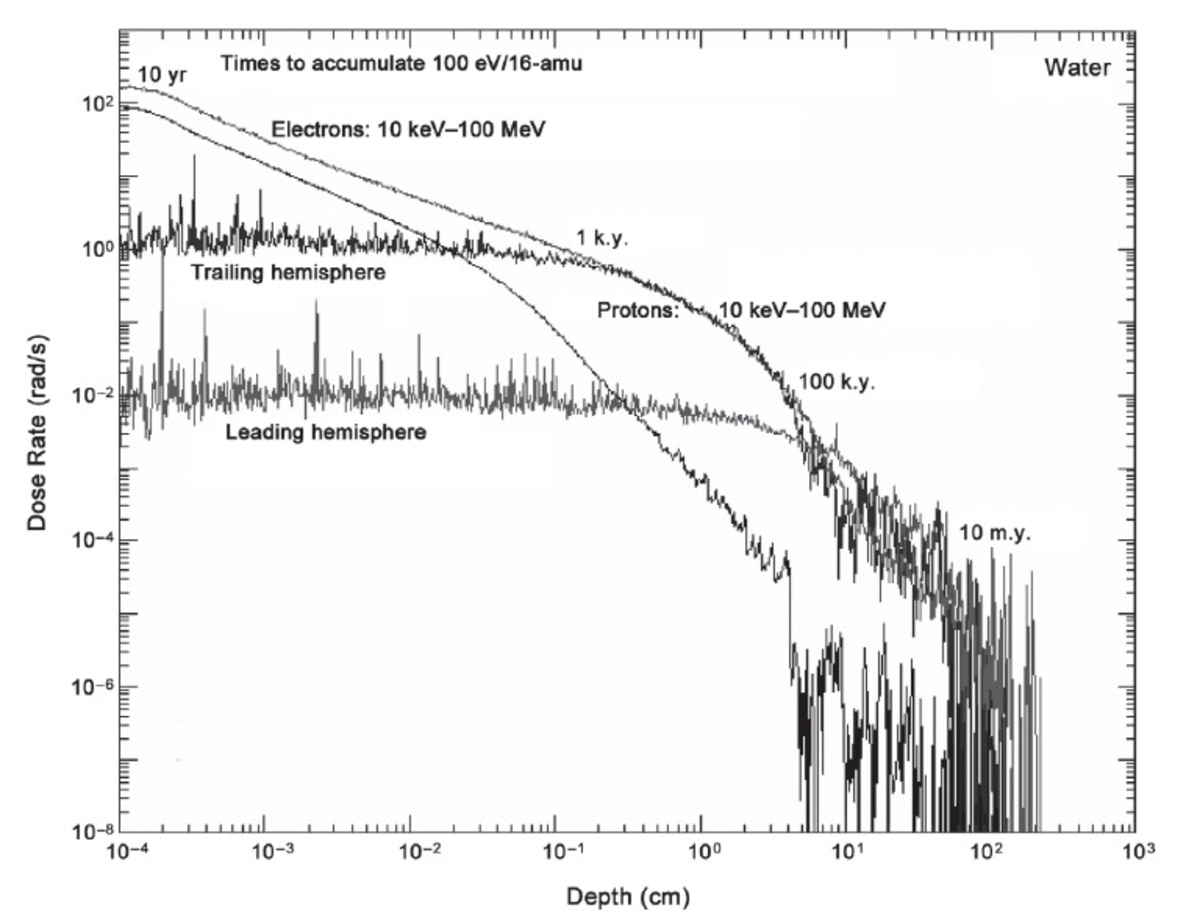
\includegraphics[scale=0.7]{figures/navtheory/icerad}
\caption{Graph from \cite{Paranicas_2009}. Shows the radiation dose rate vs. depth in the ice. The curve labeled “trailing hemisphere” includes the dose rate of 1–20 MeV electrons only, whereas the curve below it labeled leading hemisphere displays the dose rate of 20–40 MeV electrons. The two uppermost curves show the dose rate corresponding to electrons from 10 keV to 100 MeV (top curve) and the dose rate from protons between 10 keV and 100 MeV. The graph also shows times in years, that correspond to a chemically significant (most bonds
are broken at least once) dose of 60 Gigarads.}
\label{icerad}
\end{center}
\end{figure}

Since the radiation has essentially no penetration depth in the ice, the payload will only receive radiation that passes through the landing module and down the hole (the effectiveness of the Al structure as radiation shield is discussed in \ref{chap:radedl}). From this it is clear that getting the payload into the ice as quickly as possible is vital to the received radiation dose. 


\subsection{Ice melting}

The feasibility of melting the preliminary hole in the ice using a rocket engine depends on factors such as the sublimation energy of the ice vs. the energy content in the propellant, the coupling coefficient between the ice and the exhaust plume, and the ability to melt a slim deep hole that can fit the ice penetrating module in a vertical position. \\
The process can be compared to the process of oxy fuel cutting, which is used to cut thick plates of mild steel. This process is well known, and one important relationship, that is assumed to hold for ice melting as well, is the increase of the kerf with plate thickness/depth of hole. The kerf is the width of the material that is removed during cutting/melting. It is seen from table 3 in \cite{oxy_fuel}, that the kerf increases with plate thickness regardless of the width of the torch. The kerf is approximately 4\% of the plate thickness. It can very well be assumed that this ratio will be higher for ice, since the binding energy of ice is much lower than of steel. Therefore a hole of 20 cm in diameter and 2 m deep can be achieved  with a torch/jet that is substantially thinner than 20 cm. 

\subsection{Coupling coefficient and losses}
The heat in the rocket plume is energy stored in the temperature-dependent motion of particles. Heat is transferred to and from matter by the heat transfer processes (or kinetics) which are governed by the rates at which various physical phenomena occur, such as, for example, the collision rate of particles. One way to evaluate the rates that will govern the heat transfer processes during the melting of the ice, is to determine the coupling coefficient between the rocket plume and the ice. A rough estimate of the coupling coefficient has been experimentally determined during the preliminary work on our project by Lukas Christensen. The experiment was performed by melting an ice cube with a butane torch lighter. The experimental setup and calculations are shown in the Appendix \ref{app:coupling}. The obtained coupling coefficient is 0.7. It should be noted that this experiment was not conducted in vacuum, and the results might be different under other conditions. \\

\noindent
There will also be energy losses occurring from the exhaust particles that couple with the ice. The water molecules that are separated from the ice through sublimation will carry kinetic energy. This energy can either be wasted if the molecules leave the system or exploited for melting. In the beginning of the melting process most of the sublimated molecules will travel away from the system, thus wasting their energy. As the hole gets deeper, more molecules of high kinetic energy will hit the sides of the hole, instead of traveling away from the system, thereby transferring their energy to molecules in the ice and detaching them from the ice, thus helping the process along. Thus as the hole gets deeper the energy losses will decrease. Considering this along with the coupling coefficient of 0.7 a total loss of 50$\%$ of the energy from the fuel is assumed. The water vapor particles leave the hole and if possible they would deposit on the landing module making it very heavy and possibly breaking it. However, the module is heated by the RTG inside the penetrator and the water vapor molecules cannot deposit on the lander.\\
Inside the hole, the molecules from the exhaust plume and the water molecules will exert a pressure, and therefore inside the hole there will no longer be a vacuum. The pressure will narrow the plume, and it could be expected that the hole will be slimmer with depth and become triangular in shape. Not only because the jet plume will get thinner with increasing depth and thereby pressure, but also because the jet will have melted more of the ice from higher layers during the melting process. This triangular shape of the hole is not ideal, since it will off set the penetrator in a non vertical direction. More work should be done in preventing or minimizing this effect.

\subsection{Sublimation energy}

Because of the low pressure on the surface of Europa, the melted ice can not exist in its liquid phase, but will sublimate into gas phase immediately. The sublimation energy of water ice is 51059 J/mole \cite{water_prop}. One mole of water weighs 18.0155 g. The smallest amount of water that should be sublimated is a cylinder of 10 cm radius and 2 m depth. This corresponds to the volume:
\begin{equation}
\mathrm{V_{ice}}=0.1 \mathrm{m}^2 \cdot \pi \cdot 2 \mathrm{m} = 0.0628 \mathrm{m}^3
\end{equation}
The density of ice is 934 kg/m$^3$ therefore the mass of the ice cylinder is 58.7 kg. This results in $1.66\cdot 10^8$ J, needed to sublimate the cylinder shaped hole. To account for the coupling coefficient and other losses, we assume 50 \% loss of energy. This results in: $3.4 \cdot 10^8$ J. This is a fairly conservative estimate, as the losses experienced during the melting will decrease significantly as the hole gets deeper. 

\subsection{Nozzle design}

Two choices of engines have been considered for this purpose. First was to gimble the secondary engines to make them point toward the center of the lander and use them to melt the hole. This would required the engines to have a large gimbeling and throttling range, in order to assure that the lander does not tilt over or lift of the surface during the melting and to avoid stagnant flow. This option would decrease complexity and weight because of the use of already existing rockets. However the degree of gimbling and throttling that is needed might not be possible. Because we are in a near vacuum environment we should not expect to be able to throttle down to lower than 60\% of the maximum thrust without risking chugging or combustion instabilities due to the low ambient pressure. Another option is to carry an extra engine just for this purpose. The engine could be placed as close as possible to the center of the lander, right next to the hatch that will drop the descent vehicle. This engine should have a very thin jet and be turnable to avoid stagnant flow. \\

\noindent
It is difficult, if not impossible to get a thin exhaust jet in a vacuum environment, because the low ambient pressure gives rise to under expanded flows \cite{spacecraft}. Figure \ref{fig:jetflows} illustrates the issue. In low ambient pressures the exhaust plume will continue to expand past the nozzle resulting in a wide inefficient jet, as seen in figure \ref{fig:jetflows}a. The exhaust plume will expand even more  than what is seen in figure \ref{fig:jetflows}a, in the near vacuum environment of Europa. 

\begin{figure}[htb]
\begin{center}
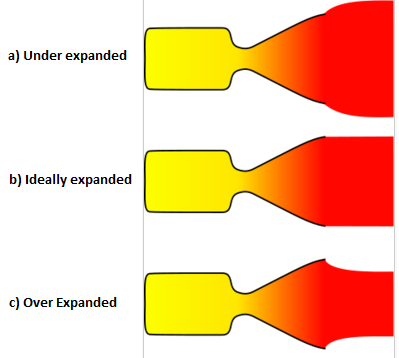
\includegraphics[scale=0.7]{figures/navtheory/nozzle}
\caption{This figure shows the effect of nozzle design on the exhaust plume. a) Under Expanded nozzle $p_e>p_a$. b) Ideally Expanded nozzle $p_e=p_a$. c) Over Expanded nozzle $p_e<p_a$. }
\label{fig:jetflows}
\end{center}
\end{figure}

The optimization of the nozzle design for operation in vacuum is evaluated through the rocket thrust equation, which is given by \cite{spacecraft}

\begin{equation}
F=mV_e+A_e(p_e-p_a)
\end{equation}

\noindent
Here $m$ is the propellant mass flow rate,  $V_e$ is the velocity of the exhaust gasses, $A_e$ is the area of nozzle exit and $p_a$ and $p_e$ is the ambient pressure and the pressure at the nozzle exit respectively. 

The incremental parameter changes are related by:
\begin{equation}
\delta F=m\delta V_e +\delta A_e(p_e-p_a) +\delta p_e A_e
\end{equation}
Because conservation of momentum states that:
\begin{equation}
m\delta V_e+\delta p_e A_e=0
\end{equation}
we get the following equation for the maximum thrust:
\begin{equation}
\dfrac{\delta F}{\delta A_e}=p_e-p_a=0 
\end{equation}

\noindent
Maximum thrust occurs when $p_e$=$p_a$, as is also seen in figure \ref{fig:jetflows}. Nozzle exit pressure, $p_a$, can be increased/decreased by smaller/larger expansion ratio, $\dfrac{A_e}{A_t}$, where $A_t$ is the area of the throat. \\
In vacuum, the thinnest theoretical jet plume and the maximum performance would be realized by an ideal nozzle with infinite exit area that would expand the combustion gases to zero pressure thereby attaining the maximum gas velocity, limited to the area below the nozzle. Therefore the best result is obtained with an engine with a large expansion ratio. This can be achieved by attaching a large nozzle to an already existing engine. Also, the kinetic energy in the jet plume should be high enough for the plume to reach the ice surface before it expands too much. 

\subsection{Energy efficiency of the rocket}
The melting will be performed using the High Performance Green Propellant which is also used for the last part of the powered landing. This is chosen because of its low toxicity in order to avoid the contamination of the ice that hydrazine would produce. Green Propellant developed by ECAPS also know as LMP-103S is a blend of Ammonium DiNitrimide (ADN), water, methanol and ammonia \cite{Walter_2014}. In formulation 60-65 \% ADN, 15-20\% methanol, 3-6\% ammonia and 9-22\% water \cite{Taylor_2013}.\\

\noindent
The thermochemical software GUIPEP is used to evaluate the energy efficiency of the propellant in regards to melting the ice. This software, developed by Arthur J. Lekstutis, can be used to calculate the theoretical performance of liquid or solid rocket propellants. The input is a list of propellant ingredients (and the mass of each), as well as chamber pressure and ambient pressure. The output includes average exhaust Energy and velocity \cite{GUIPEP}. \\

\noindent
The energy efficiency of the propellant in low pressure environment depending on the chamber pressure of the engine has been calculated using GUIPEP. The results are shown in fig \ref{guigraf}. The results show that theoretically the highest amount of energy that can be obtained from the propellant is 2.74 kJ/g. Thus, from these calculations, a minimum amount of 124 kg HPGP is needed to melt/sublimate the hole.  This is a significant amount of extra weight for the lander, and since the exact amount of fuel needed for the final phase of the landing i not known, we must accept to use whatever fuel is left in the tanks after landing.\\
\begin{figure}[htb]
\begin{center}
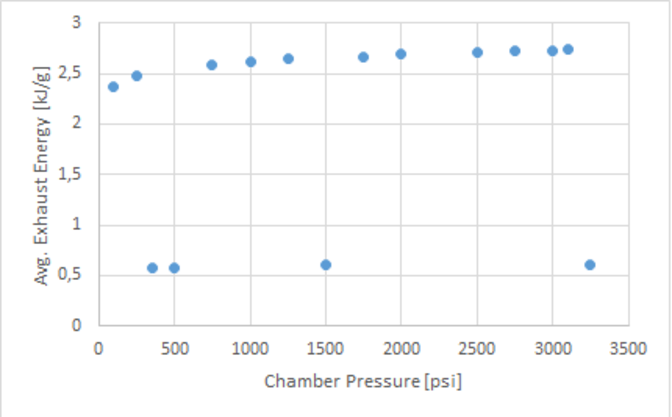
\includegraphics[scale=0.8]{figures/navtheory/guigraf}
\caption{Graph showing the average energy in the exhaust plume in kJ/g depending on the chamber pressure, calculated using GUIPEP.}
\label{guigraf}
\end{center}
\end{figure}

\noindent
The results shown in figure \ref{guigraf} should be taken into consideration along with the the previously mentioned optimization of expansion ratio, which can be achieved with a long nozzle, when choosing or designing a suitable engine. Also the engine should be turnable in the low pressure to avoid stagnant flow and to be efficient for all depths of the hole. A thruster from ECAPS could be an option. ECAPS has built and tested more than 60 HPGP thrusters with thrust levels ranging from 0.5 N to 220 N. The technology has been demonstrated in-space in the propulsion system for the PRISMA mission launched in 2009 \cite{Walter_2014}.
